\documentclass[12pt,a4paper]{article}

\usepackage[utf8]{inputenc}
\usepackage[T1]{fontenc}
\usepackage[spanish,es-tabla]{babel}
\usepackage{newtxtext}
\usepackage{newtxmath}
\usepackage{geometry}
\usepackage{graphicx}
\usepackage{booktabs}
\usepackage{array}
\usepackage[table]{xcolor}
\usepackage{tikz}
\usetikzlibrary{arrows.meta,positioning,babel}
\usepackage{hyperref}
\usepackage{xurl}
\usepackage{csquotes}
\usepackage[backend=biber,style=ieee,sorting=none]{biblatex}

\geometry{top=2.5cm,bottom=2.5cm,left=2.5cm,right=2.5cm}
\addbibresource{referencias.bib}
\hypersetup{
  colorlinks=true,
  linkcolor=black,
  citecolor=black,
  urlcolor=blue,
  pdftitle={Análisis crítico de Apache Hadoop HDFS}
}

\begin{document}

\begin{titlepage}
  \centering
  \vspace*{1.5cm}
  {\Large\textbf{Universidad Técnica Estatal de Quevedo}\par}
  \vspace{0.5cm}
  {\large Facultad de Ciencias de la Ingeniería\par}
  {\large Carrera de Ingeniería de Software\par}

  \vspace{1.8cm}
  {\large\textbf{Asignatura:} Sistemas Distribuidos\par}
  \vspace{0.3cm}
  {\large\textbf{Actividad:} TA-IND-01 --- Informe Académico Individual\par}

  \vspace{1.8cm}
  {\LARGE\textbf{Análisis crítico de Apache Hadoop HDFS y comparación con Ceph}\par}

  \vspace{1.8cm}
  {\large\textbf{Estudiante:} Steven Fernando Pozo Castillo\par}
  {\large\textbf{Curso/Paralelo:} Séptimo semestre ``B''\par}
  {\large\textbf{Fecha:} 14 de noviembre de 2026\par}

  \vfill
  {\large\textbf{Repositorio público:}\par}
  \vspace{0.2cm}
  {\small\url{https://github.com/Redsito1215/TA-IND-01-Apache-Hadoop-HDFS-comparado-con-Ceph}\par}
\end{titlepage}

\begin{abstract}
Este informe analiza Apache Hadoop Distributed File System (HDFS), un sistema de archivos distribuido utilizado para almacenar grandes volúmenes de información en varios equipos. El estudio se concentra en la función del NameNode, la distribución de bloques entre DataNodes y la replicación como mecanismo de tolerancia a fallos. Los conceptos de transparencia, comunicación, CAP y PACELC se aplican a la arquitectura real, evitando tratar a HDFS como si fuera una base de datos transaccional. Además, se realiza una prueba local con Docker formada por un NameNode y tres DataNodes. En ella se almacena un archivo con factor de replicación tres, se pausa uno de los nodos y se comprueba que la lectura continúa desde otra copia. Los resultados se contrastan con Ceph, que distribuye la ubicación de objetos mediante CRUSH y evita depender de un único servicio equivalente al NameNode para resolver cada acceso. Se concluye que HDFS ofrece una solución sencilla y resistente para archivos grandes y procesamiento por lotes, aunque la centralización de metadatos y el costo de mantener varias copias limitan su conveniencia en cargas con muchos archivos pequeños o acceso de baja latencia.
\end{abstract}

\section{Introducción}

Apache Hadoop HDFS resuelve el problema de almacenar archivos que superan la capacidad o la confiabilidad de un solo servidor. En lugar de guardar cada archivo completo en una máquina, lo divide en bloques y distribuye copias entre varios DataNodes. Este enfoque se utiliza principalmente en ambientes de Big Data, donde los datos se procesan de forma paralela y resulta más importante mantener un flujo alto de lectura que responder en pocos milisegundos.

La elección de HDFS se debe a que su tolerancia a fallos puede observarse en un equipo personal. Un clúster pequeño permite identificar la relación entre el NameNode y los DataNodes, revisar la ubicación de un bloque y provocar la pérdida temporal de respuesta de una réplica. Además, su diseño presenta un contraste claro con Ceph. HDFS mantiene los metadatos del sistema de archivos en el NameNode, mientras Ceph calcula la ubicación de los objetos mediante el algoritmo CRUSH y una estructura de almacenamiento más descentralizada.

La literatura reciente muestra que la replicación fija de HDFS mantiene la disponibilidad, pero también puede desperdiciar espacio cuando se aplica por igual a archivos con patrones de uso diferentes \cite{tlich2025replication}. Asimismo, la concentración de metadatos en el NameNode puede convertirse en un límite de escalabilidad, motivo por el cual se han estudiado técnicas como la federación y el particionamiento del espacio de nombres \cite{dhulavvagol2023federation}.

\section{Arquitectura del sistema}

La arquitectura básica de HDFS sigue un modelo maestro-trabajador. El NameNode administra el espacio de nombres, los permisos, la relación entre archivos y bloques, y la ubicación de las réplicas. Los DataNodes almacenan físicamente los bloques y atienden las operaciones de lectura y escritura solicitadas por los clientes.

Cuando un cliente desea leer un archivo, primero consulta al NameNode para obtener las ubicaciones de sus bloques. Después se comunica directamente con los DataNodes, sin hacer pasar el contenido por el NameNode. En una escritura, el NameNode selecciona una cadena de DataNodes y el bloque circula por esa cadena hasta completar el número de réplicas configurado. Esta separación evita que el servidor de metadatos cargue con todo el tráfico de datos, aunque mantiene una dependencia importante respecto de su disponibilidad.

Los DataNodes envían \textit{heartbeats} y reportes de bloques al NameNode. Los primeros indican que continúan activos; los segundos permiten conocer qué bloques conserva cada nodo. Si el NameNode deja de recibir señales de un DataNode, lo marca como no disponible y programa nuevas copias de los bloques que hayan quedado por debajo del factor de replicación. La replicación mejora la confiabilidad y el acceso, pero consume capacidad y tráfico de red \cite{swaroopa2023replication}.

El clúster del experimento reproduce esta estructura con cuatro contenedores: un NameNode y tres DataNodes conectados a una red privada de Docker. El archivo de prueba se almacena con factor de replicación tres, por lo que cada DataNode conserva una copia del único bloque generado.

\begin{figure}[htbp]
  \centering
  \begin{tikzpicture}[
    node distance=1.3cm and 1.6cm,
    componente/.style={draw, rounded corners, align=center, minimum width=3.1cm,
      minimum height=1.05cm, fill=blue!8},
    datos/.style={draw, rounded corners, align=center, minimum width=3.1cm,
      minimum height=1.05cm, fill=green!10},
    enlace/.style={-Latex, thick},
    doble/.style={<->, >=Latex, thick}
  ]
    \node[componente] (cliente) {Cliente HDFS\\\small rutas y comandos};
    \node[componente, right=of cliente] (namenode) {NameNode\\\small metadatos y ubicación};

    \node[datos, below=1.8cm of namenode, xshift=-4.0cm] (dn1) {DataNode 1\\\small réplica del bloque};
    \node[datos, below=1.8cm of namenode] (dn2) {DataNode 2\\\small réplica del bloque};
    \node[datos, below=1.8cm of namenode, xshift=4.0cm] (dn3) {DataNode 3\\\small réplica del bloque};

    \draw[doble] (cliente) -- node[above, align=center]{\small RPC\\\small consulta de metadatos} (namenode);
    \draw[enlace] (namenode) -- node[left, sloped]{\small ubicación} (dn1);
    \draw[enlace] (namenode) -- node[right]{\small control} (dn2);
    \draw[enlace] (namenode) -- node[right, sloped]{\small ubicación} (dn3);

    \draw[doble, dashed] (cliente.south) -- ++(0,-1.0) -| node[pos=0.72, below]{\small lectura/escritura TCP} (dn1.west);
    \draw[enlace, orange!80!black] (dn1) -- node[below]{\small réplica 2} (dn2);
    \draw[enlace, orange!80!black] (dn2) -- node[below]{\small réplica 3} (dn3);

    \node[below=0.7cm of dn2, align=center, text width=11cm] (nota)
      {\small Los DataNodes envían \textit{heartbeats} y reportes de bloques al NameNode.\\
       El contenido circula directamente entre cliente y DataNodes; el NameNode no transporta los bloques.};
  \end{tikzpicture}
  \caption{Arquitectura simplificada del clúster HDFS utilizado en el experimento.}
  \label{fig:arquitectura-hdfs}
\end{figure}


\section{Análisis con los conceptos de la Unidad 1}

\subsection{Transparencias de distribución}

HDFS proporciona transparencia de acceso porque el usuario trabaja con rutas y comandos semejantes a los de un sistema de archivos, sin indicar manualmente en qué DataNode se encuentra cada bloque. También ofrece transparencia de ubicación y replicación: el cliente consulta una ruta lógica y el NameNode devuelve las réplicas disponibles. La ubicación física puede cambiar después de una recuperación o un balanceo sin modificar el nombre utilizado por la aplicación.

La transparencia de fallos es parcial. Cuando una réplica no responde, el cliente puede leer desde otra copia. Sin embargo, una caída del NameNode activo, una demora en la detección del fallo o una partición que impida alcanzar una mayoría de servicios de coordinación puede hacerse visible como una pausa o un error. HDFS tampoco oculta por completo los problemas de concurrencia. Está optimizado para escribir una vez y leer muchas veces; no ofrece el mismo tipo de actualización concurrente y aleatoria que un sistema de archivos local de propósito general.

\subsection{CAP y PACELC}

HDFS no es una base de datos y su clasificación CAP debe aplicarse con cuidado. En la capa de metadatos, el sistema prioriza una visión coherente del espacio de nombres. Si el NameNode activo no puede operar o no existe un reemplazo disponible, las nuevas operaciones se detienen antes que permitir cambios contradictorios. Por esta razón, su comportamiento se aproxima a una preferencia por consistencia frente a disponibilidad durante una partición.

En ausencia de particiones, HDFS acepta latencias mayores con el fin de conservar redundancia. Una escritura puede recorrer varios DataNodes antes de ser reconocida, mientras las lecturas intentan elegir una réplica cercana. Desde PACELC, esta decisión se aproxima a favorecer consistencia y durabilidad sobre una latencia mínima. No obstante, el resultado depende de la configuración del clúster, del factor de replicación y de si se utiliza alta disponibilidad para el NameNode.

\subsection{Modelos de comunicación}

El sistema combina varios mecanismos. La consulta de metadatos sigue un modelo cliente-servidor mediante RPC entre el cliente y el NameNode. La transferencia del contenido ocurre directamente entre el cliente y los DataNodes mediante conexiones TCP. Durante la escritura, los DataNodes forman una tubería para reenviar el bloque y confirmar su recepción.

La comunicación de control es periódica y asíncrona. Los heartbeats y reportes de bloques permiten al NameNode actualizar su visión del clúster sin consultar continuamente cada servidor. Por tanto, HDFS no es completamente \textit{peer-to-peer}: conserva coordinación central para los metadatos y distribución directa para los datos.

\subsection{Tolerancia a fallos}

La principal defensa de HDFS frente a fallos es almacenar varias copias de cada bloque. Si un DataNode deja de responder, el NameNode puede seleccionar otra ubicación y ordenar una nueva réplica. Los clientes también pueden cambiar de réplica cuando una lectura falla. A esto se añaden sumas de verificación para detectar bloques dañados y configuraciones de alta disponibilidad con un NameNode activo y otro en espera.

La tolerancia no es gratuita. Aumentar el número de copias eleva el uso de disco y el tráfico durante las escrituras. Las investigaciones recientes buscan ajustar la cantidad de réplicas según la frecuencia de acceso y la importancia del archivo, en lugar de aplicar el mismo valor a todos los datos \cite{tlich2025replication}. En términos generales, la tolerancia a fallos requiere equilibrar disponibilidad, rendimiento y consumo de recursos \cite{saadoon2022fault}.

\section{Experimentación propia}

La prueba se realizó en Docker con un NameNode y tres DataNodes conectados a la red privada \texttt{ta-ind-01-hdfs-network}. Se creó el archivo \texttt{archivo\_estudiante.txt}, de 241 bytes, y se almacenó en la ruta \texttt{/ta-ind-01/}. La configuración estableció un factor de replicación tres.

Antes de provocar el fallo se ejecutó \texttt{hdfs fsck} para comprobar la ubicación del bloque. La salida indicó un bloque en estado \texttt{OK}, tres réplicas vivas, cero bloques perdidos y estado general \texttt{HEALTHY}. Esto confirmó que cada DataNode conservaba una copia del archivo.

Luego se pausó \texttt{hdfs-taind-datanode1}. La pausa mantuvo el contenedor conectado a la red, pero impidió que respondiera. Para evitar que el cliente permaneciera esperando indefinidamente se configuró un tiempo de espera de tres segundos. La lectura con \texttt{hdfs dfs -cat} terminó correctamente y mostró el contenido completo del archivo. Finalmente se reactivó el nodo y una segunda ejecución de \texttt{fsck} volvió a mostrar tres réplicas vivas y ningún bloque perdido.

\begin{table}[htbp]
  \centering
  \caption{Resultados observados durante el experimento}
  \label{tab:resultados}
  \renewcommand{\arraystretch}{1.25}
  \begin{tabular}{p{3.2cm}p{3.1cm}p{6.5cm}}
    \toprule
    \textbf{Fase} & \textbf{Resultado} & \textbf{Interpretación} \\
    \midrule
    Estado inicial & 3 réplicas, \texttt{HEALTHY} & El bloque estaba disponible en los tres DataNodes. \\
    Nodo pausado & \texttt{datanode1} sin respuesta & El clúster conservó dos copias accesibles. \\
    Lectura degradada & Lectura correcta & El cliente obtuvo el bloque desde otra réplica. \\
    Recuperación & 3 réplicas, \texttt{HEALTHY} & El nodo volvió a participar sin perder el archivo. \\
    \bottomrule
  \end{tabular}
\end{table}

La prueba valida la tolerancia de lectura frente a un nodo sin respuesta, pero tiene límites. Todos los contenedores se ejecutaron en el mismo equipo, por lo que no representan fallos físicos independientes ni una partición real entre centros de datos. Tampoco se midió la reconstrucción de archivos grandes. El resultado demuestra el mecanismo básico de selección de réplicas, no el rendimiento de un clúster de producción.

Las figuras siguientes registran la ejecución real. Primero se comprobó que los cuatro contenedores estaban activos y que el NameNode reconocía tres DataNodes. Después, la salida de \texttt{fsck} confirmó las tres réplicas. Por último, Docker Desktop mostró el primer DataNode pausado mientras los otros dos y el NameNode continuaban activos.

\begin{figure}[htbp]
  \centering
  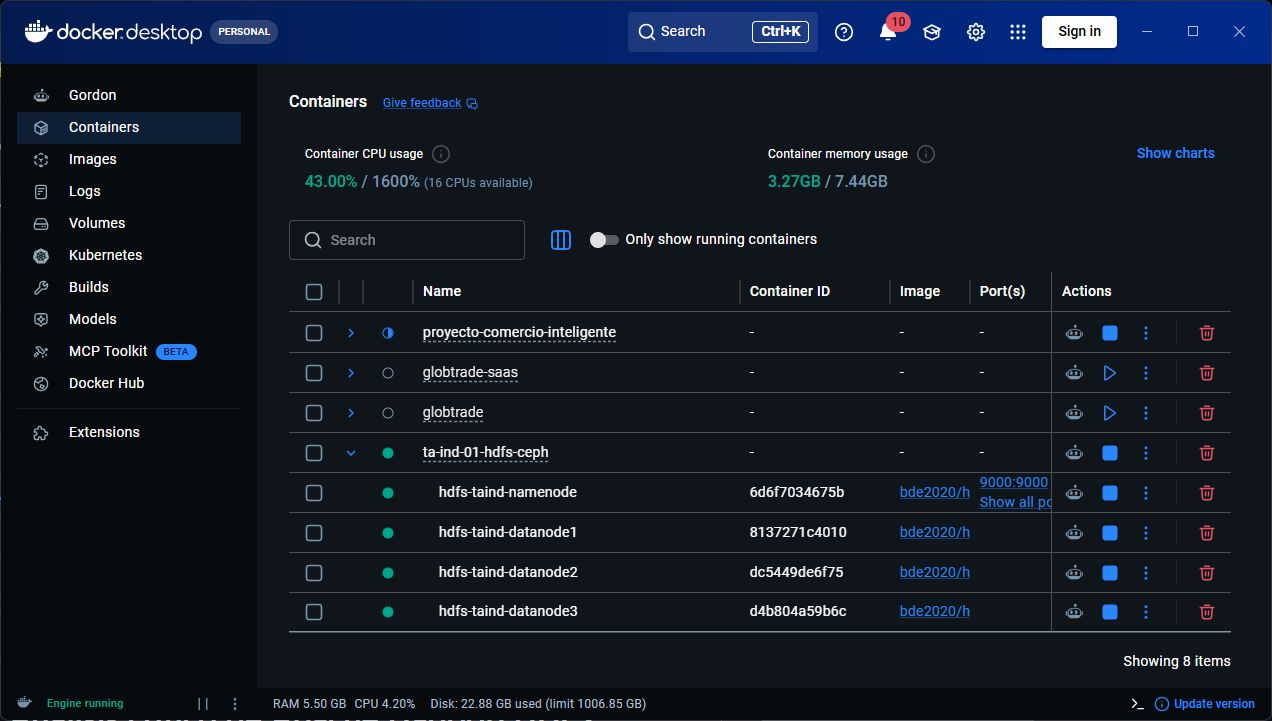
\includegraphics[width=0.95\linewidth]{../figuras/01_contenedores_activos.png}
  \caption{NameNode y tres DataNodes activos en Docker Desktop.}
  \label{fig:contenedores-activos}
\end{figure}

\begin{figure}[htbp]
  \centering
  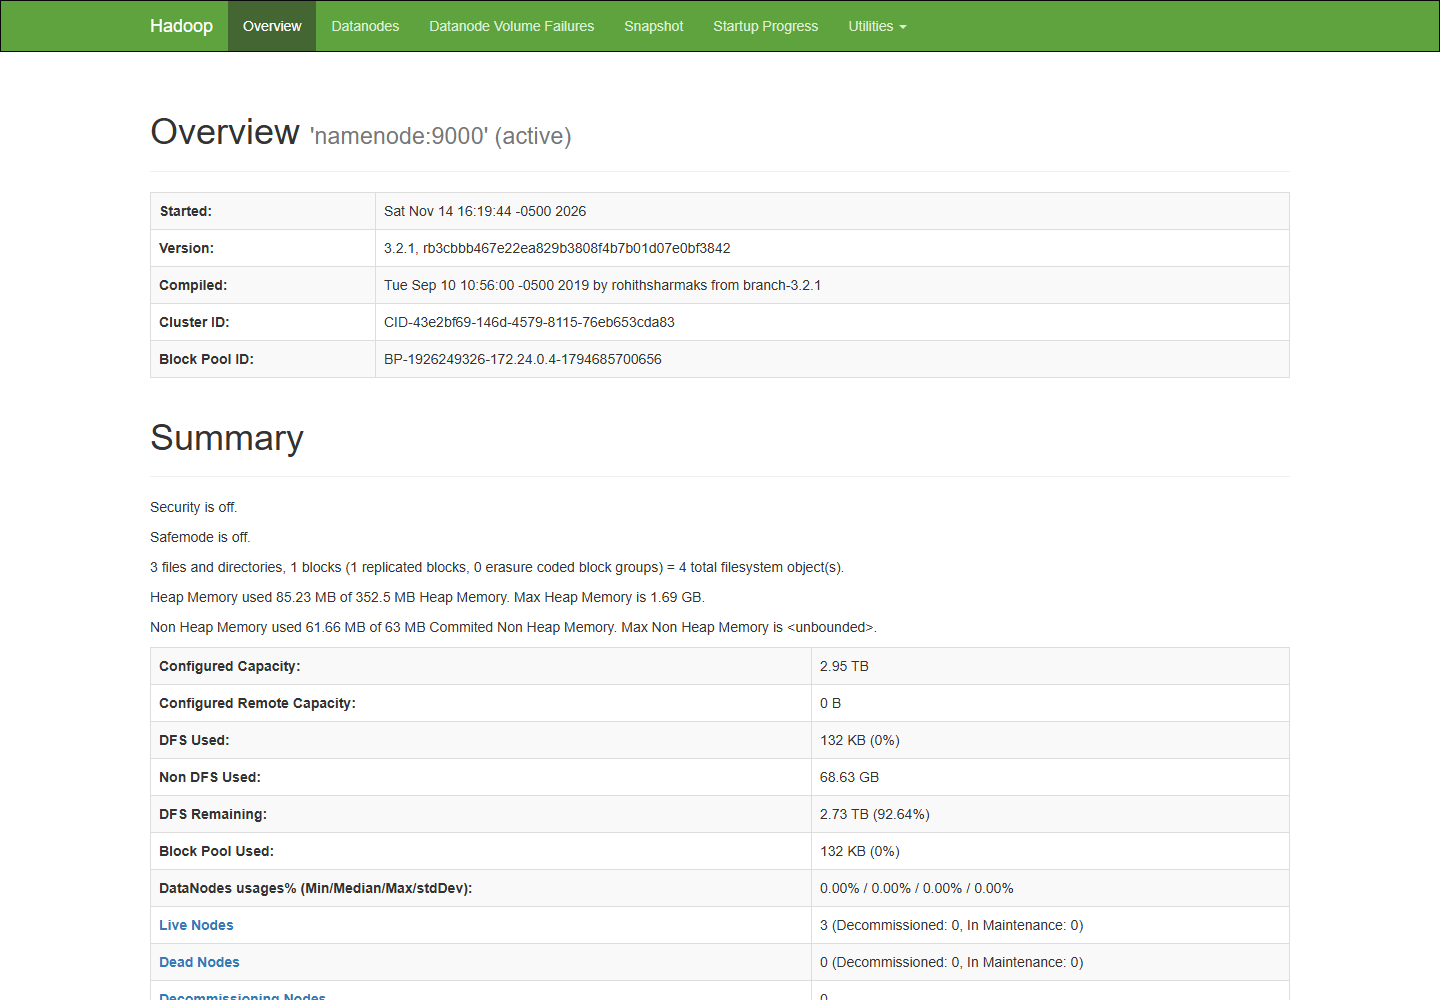
\includegraphics[width=0.95\linewidth]{../figuras/02_estado_namenode.png}
  \caption{Resumen del NameNode con tres nodos vivos y ningún nodo caído.}
  \label{fig:estado-namenode}
\end{figure}

\begin{figure}[htbp]
  \centering
  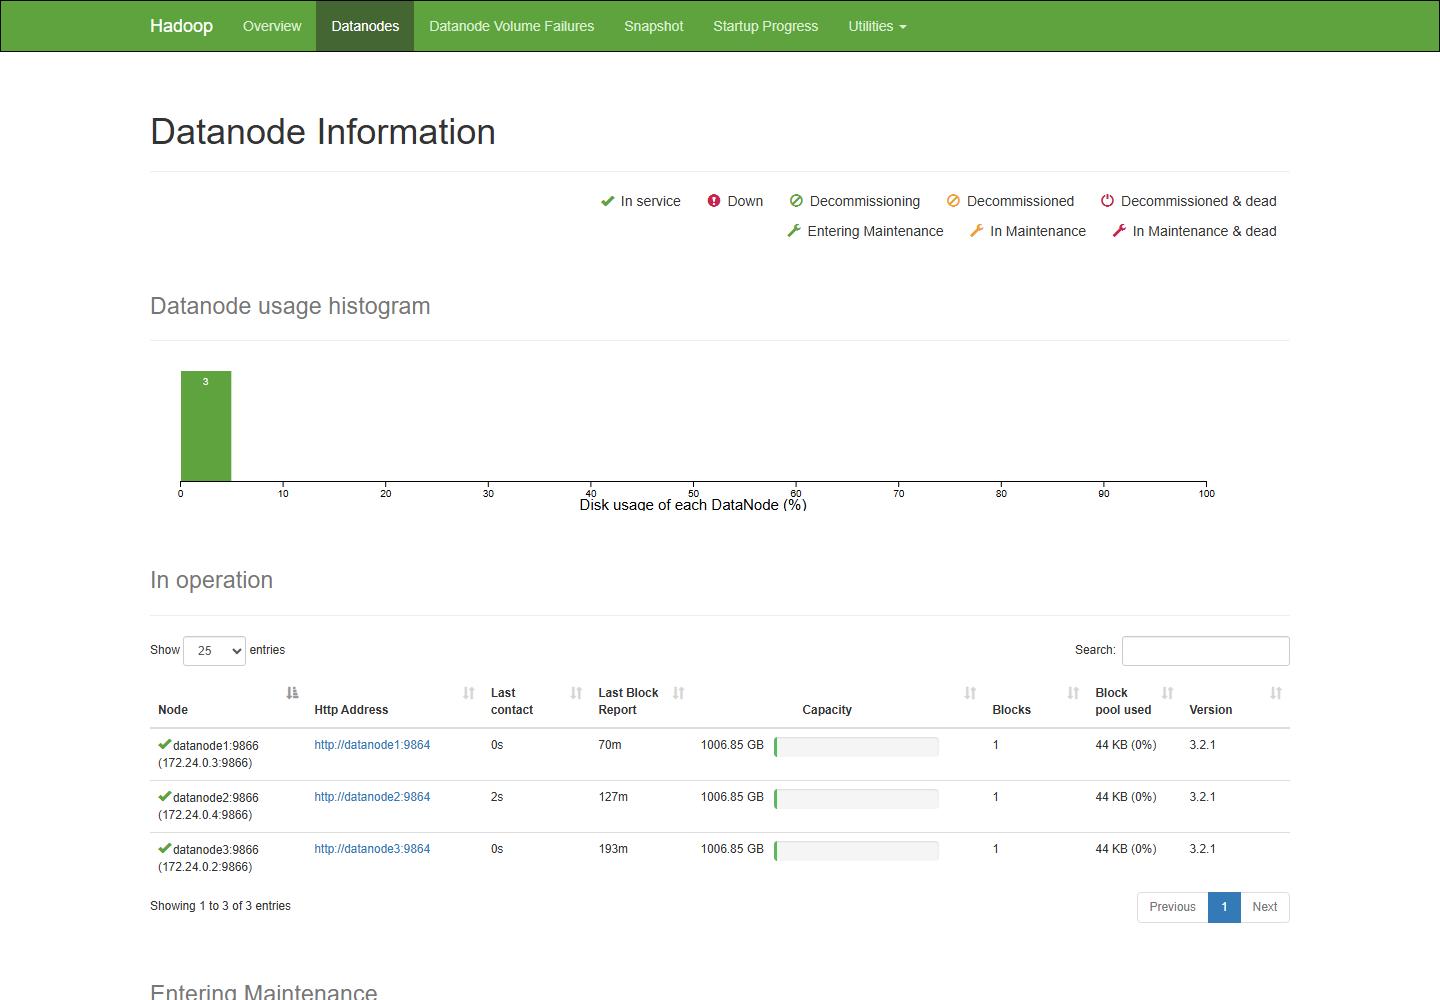
\includegraphics[width=0.95\linewidth]{../figuras/03_tres_datanodes.png}
  \caption{Los tres DataNodes en operación y con una copia del bloque.}
  \label{fig:tres-datanodes}
\end{figure}

\begin{figure}[htbp]
  \centering
  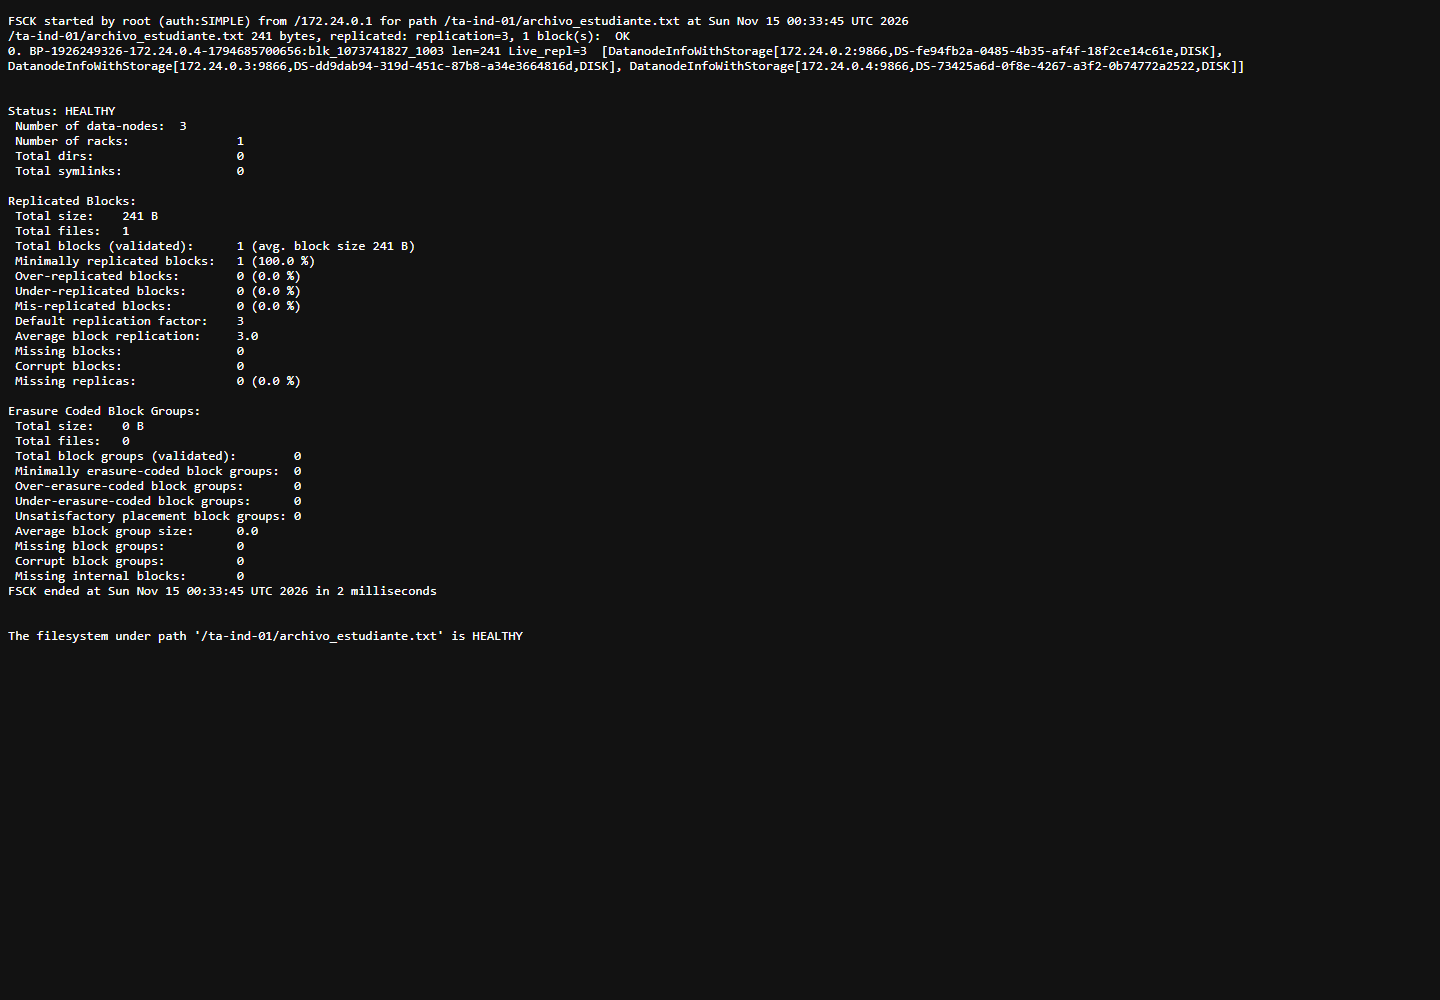
\includegraphics[width=0.95\linewidth]{../figuras/04_replicacion_fsck.png}
  \caption{Comprobación del archivo con factor de replicación tres y estado saludable.}
  \label{fig:replicacion-fsck}
\end{figure}

\begin{figure}[htbp]
  \centering
  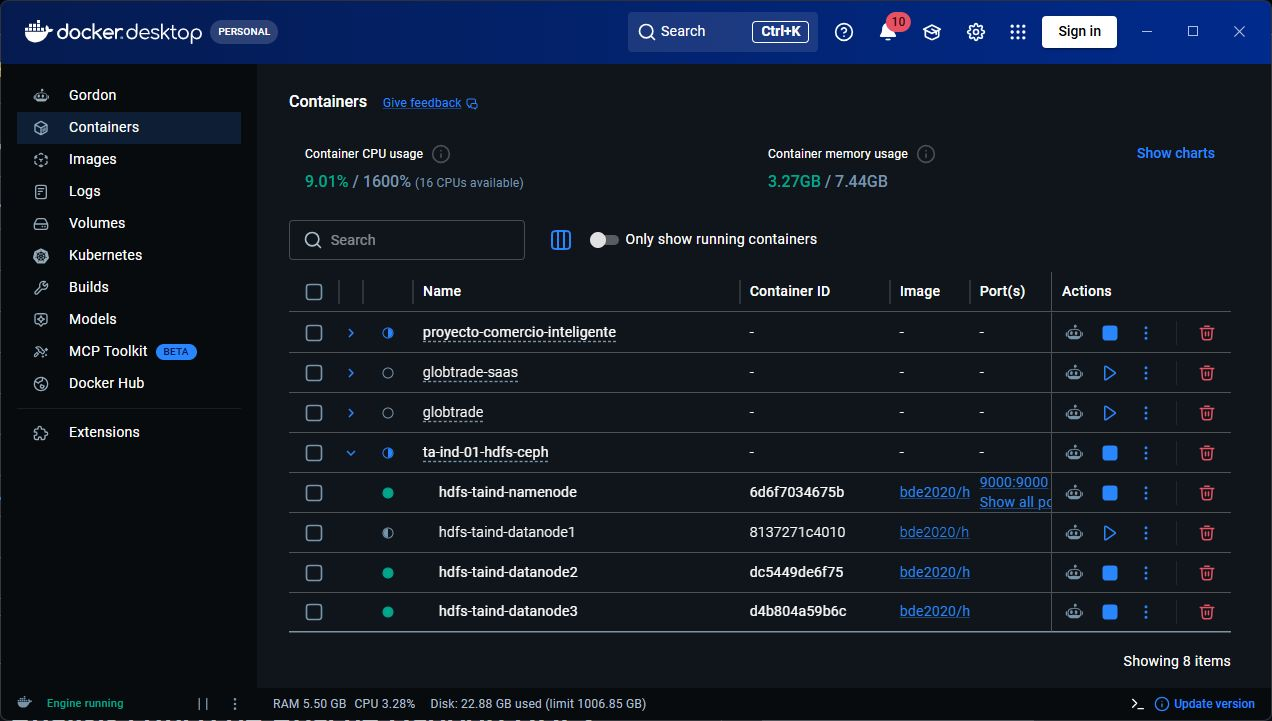
\includegraphics[width=0.95\linewidth]{../figuras/05_datanode_pausado.png}
  \caption{DataNode 1 pausado mientras los demás componentes permanecen activos.}
  \label{fig:datanode-pausado}
\end{figure}

Las capturas de terminal complementan la interfaz gráfica y permiten comprobar la autoría de la ejecución mediante el usuario, el nombre del equipo y la fecha del sistema. También conservan los comandos utilizados y la salida obtenida sin modificarla.

\begin{figure}[htbp]
  \centering
  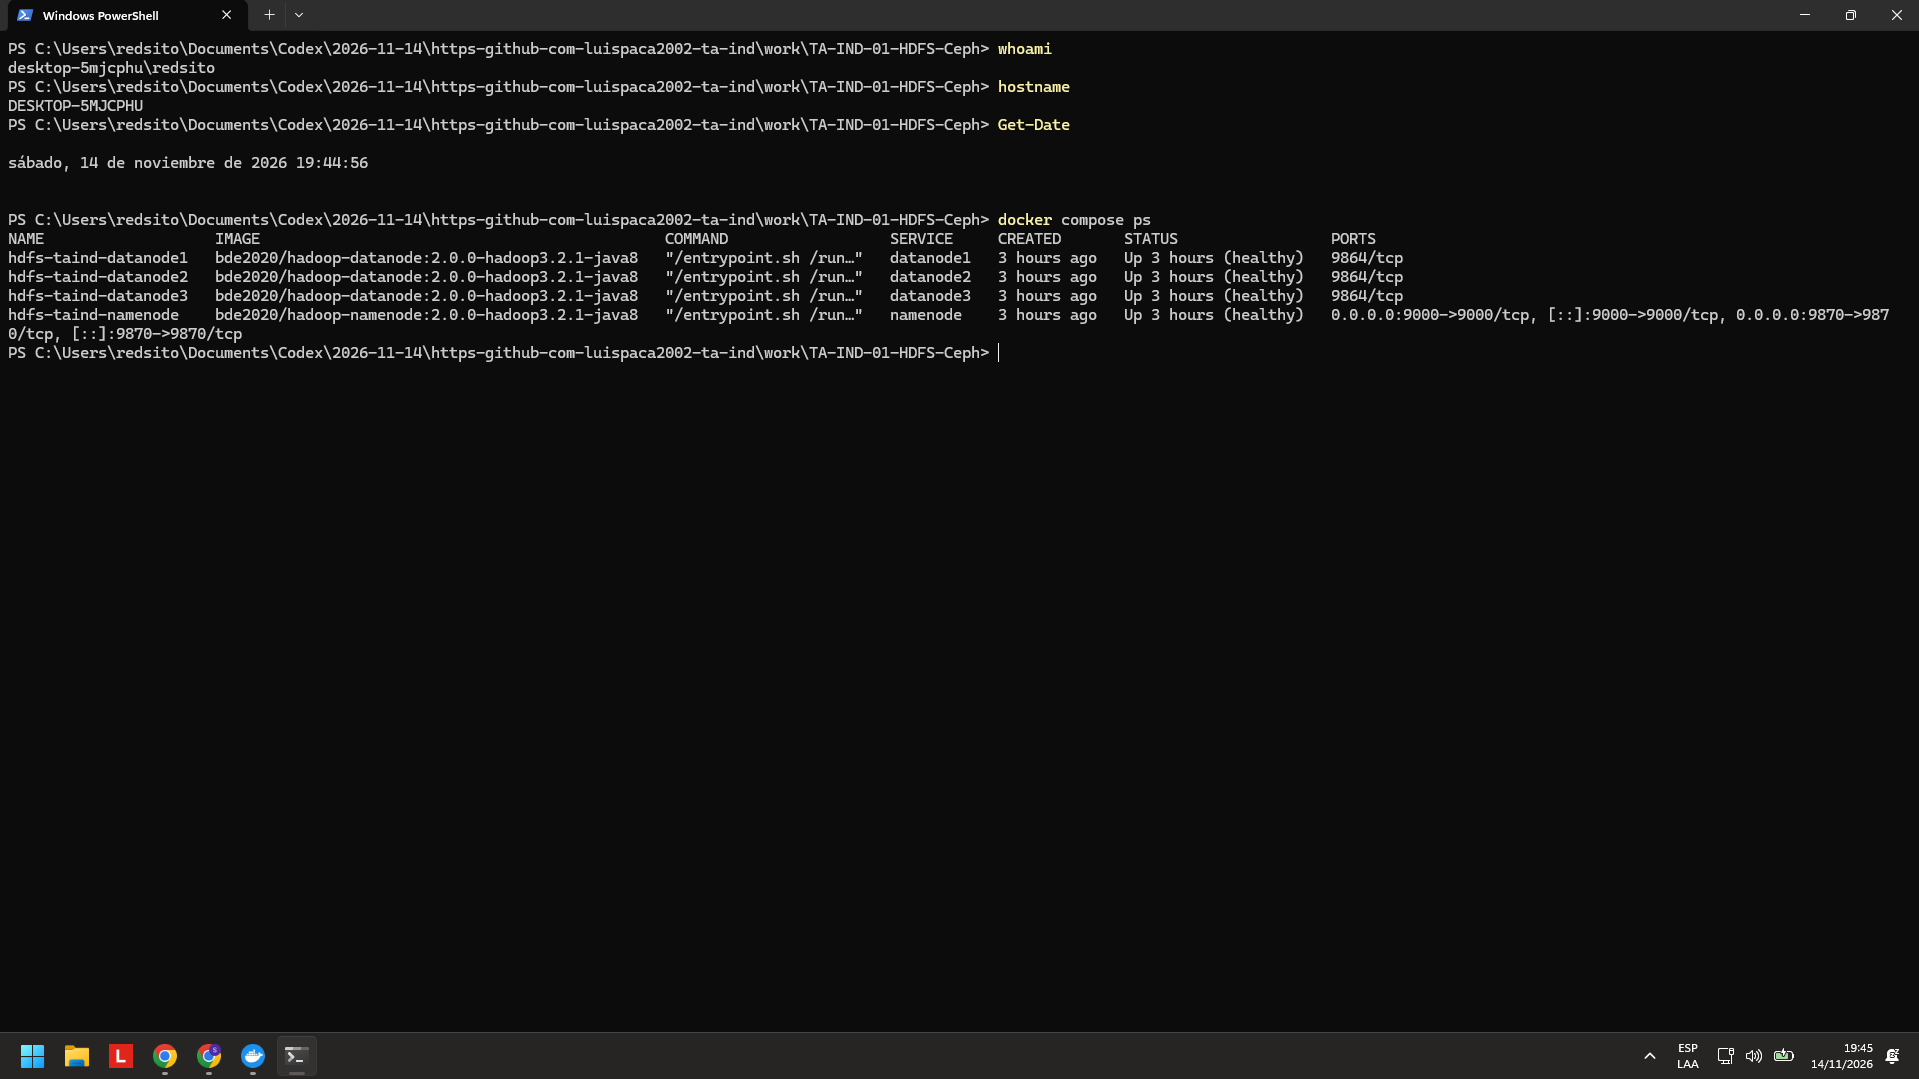
\includegraphics[width=0.95\linewidth]{../figuras/06_terminal_contenedores.png}
  \caption{Datos de la sesión y cuatro contenedores activos en la terminal.}
  \label{fig:terminal-contenedores}
\end{figure}

\begin{figure}[htbp]
  \centering
  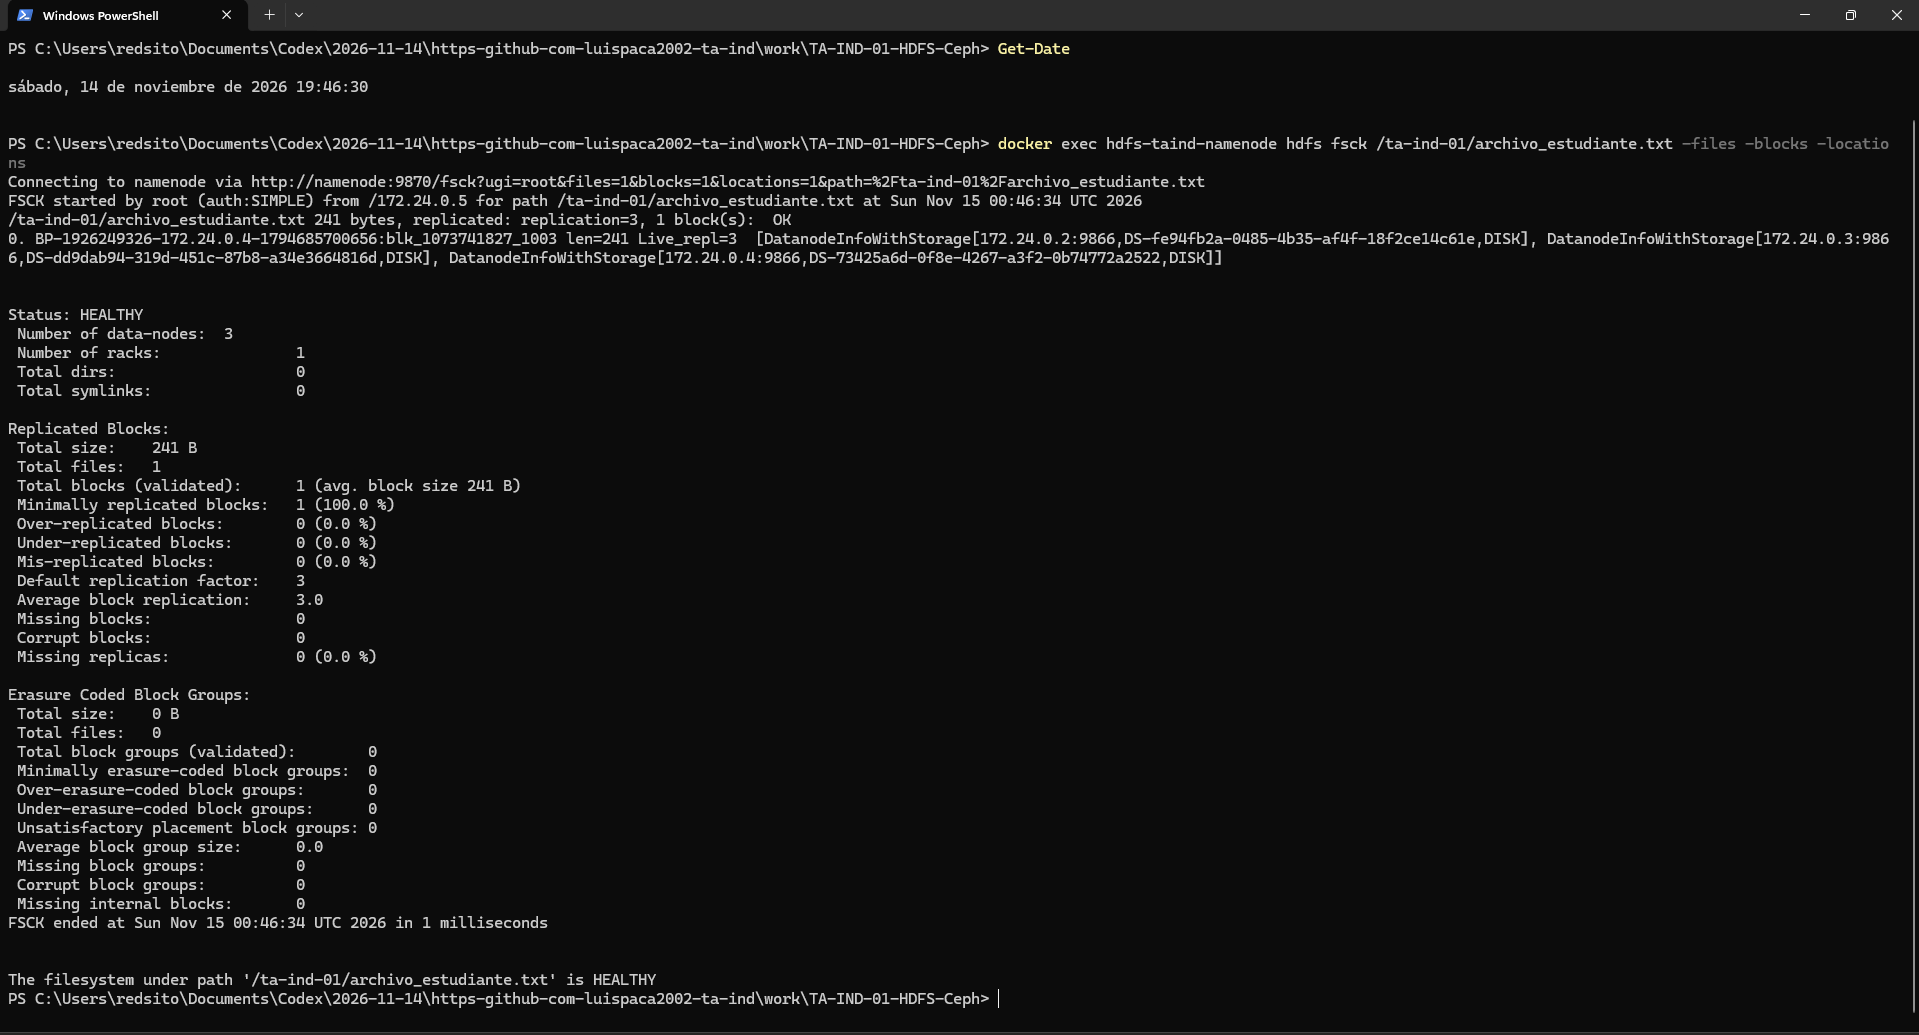
\includegraphics[width=0.95\linewidth]{../figuras/07_terminal_replicacion.png}
  \caption{Salida de \texttt{fsck}: tres réplicas vivas y sistema de archivos saludable.}
  \label{fig:terminal-replicacion}
\end{figure}

\begin{figure}[htbp]
  \centering
  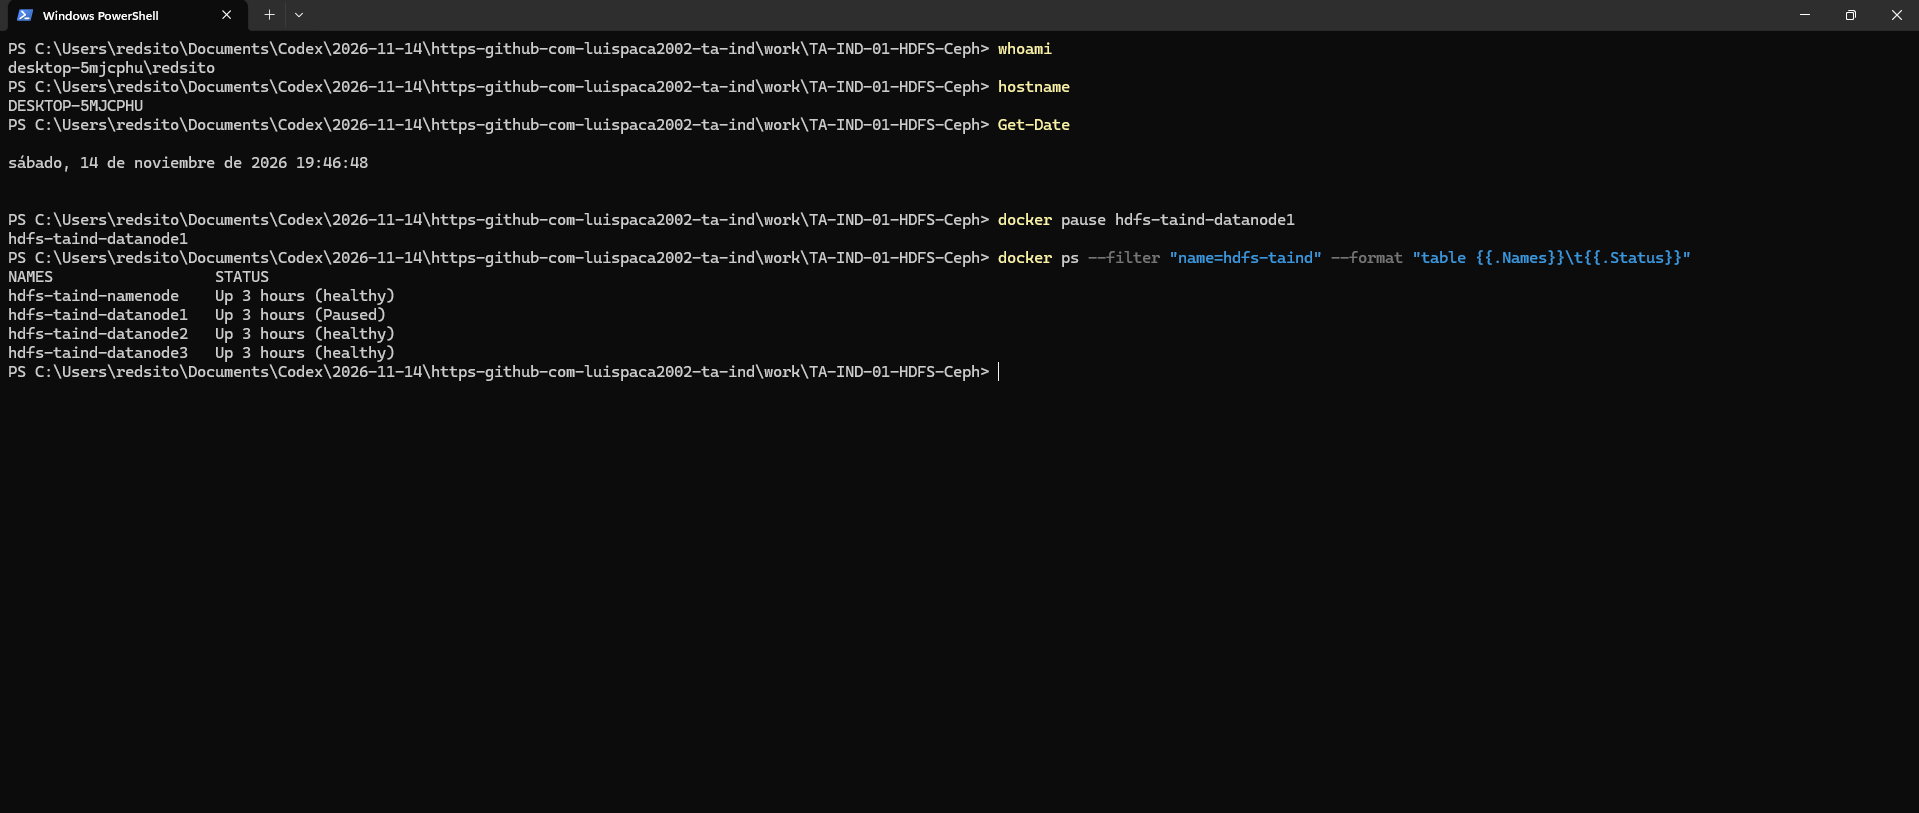
\includegraphics[width=0.95\linewidth]{../figuras/08_terminal_nodo_pausado.png}
  \caption{Identificación de la sesión y estado pausado del primer DataNode.}
  \label{fig:terminal-nodo-pausado}
\end{figure}

\begin{figure}[htbp]
  \centering
  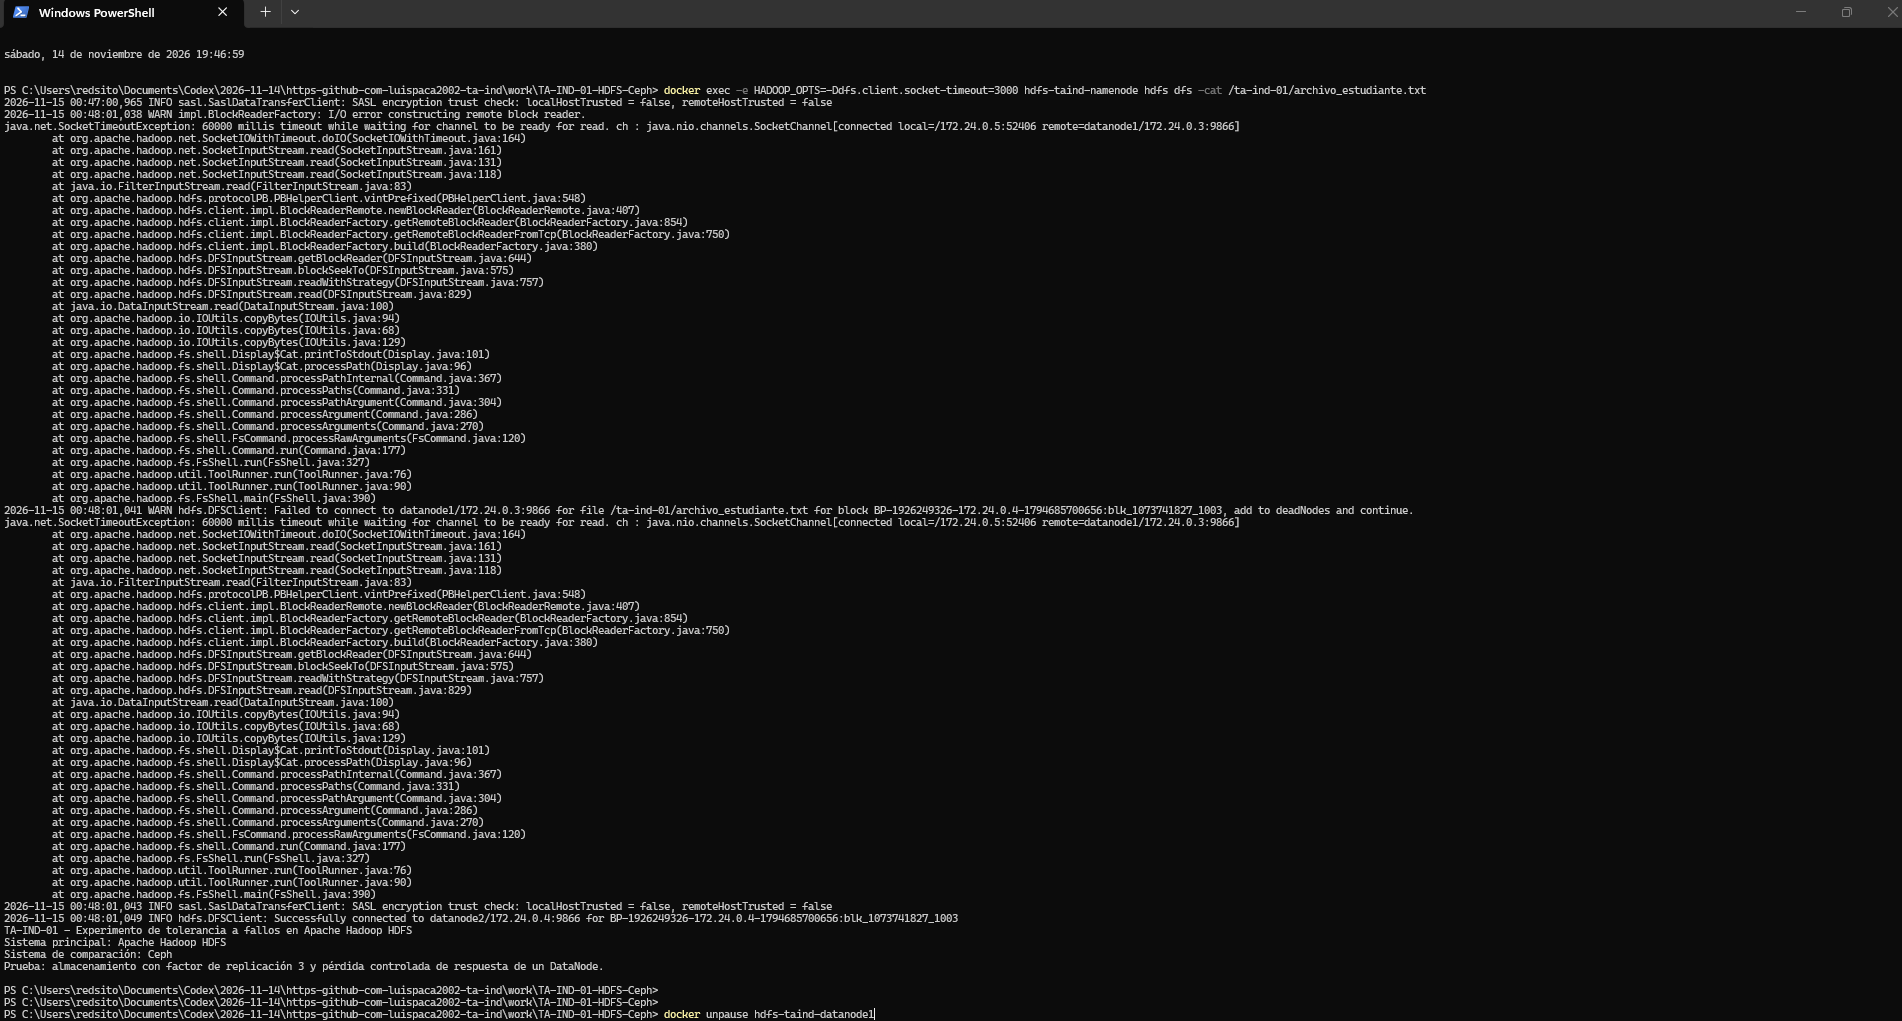
\includegraphics[width=0.95\linewidth]{../figuras/09_terminal_lectura_fallo.png}
  \caption{Fallo de la primera réplica y lectura completada desde otro DataNode.}
  \label{fig:terminal-lectura-fallo}
\end{figure}

\section{Ejemplos del entorno personal}

\subsection{SGA de la UTEQ}

He observado que el SGA puede volverse lento o presentar dificultades de acceso cuando se acerca una fecha de entrega. Como usuario no puedo conocer su arquitectura interna, pero el comportamiento permite relacionar la experiencia con la concurrencia y la disponibilidad. Muchas solicitudes llegan en un intervalo corto y aumentan el tiempo de respuesta. Si un servicio central se satura, la distribución de componentes no es transparente para el estudiante porque la demora se vuelve visible. Este caso muestra que un sistema distribuido no se evalúa solo por almacenar copias; también necesita repartir carga y conservar capacidad durante los picos.

\subsection{WhatsApp durante una pérdida de conexión}

En WhatsApp he visto mensajes que quedan pendientes cuando falla la conexión y se envían o sincronizan después. Esta experiencia se relaciona con comunicación asíncrona y tolerancia a desconexiones temporales. La aplicación conserva el mensaje localmente y reintenta la entrega cuando vuelve a existir conectividad. Para el usuario existe una transparencia parcial: no debe escribir nuevamente el contenido, pero los indicadores de estado muestran que todavía no llegó al servidor o al destinatario. A diferencia de HDFS, el objetivo principal no es recuperar un bloque replicado, sino mantener la entrega y el orden de mensajes mientras cambia la conectividad.

\section{Análisis comparativo con Ceph}

Ceph resuelve el almacenamiento distribuido con una arquitectura diferente. Sus clientes utilizan el mapa del clúster y el algoritmo CRUSH para calcular la ubicación de los objetos. De esta manera, la ruta de los datos no depende de consultar un NameNode para cada bloque. Los OSD almacenan los objetos y participan en replicación, recuperación y balanceo. Trabajos recientes muestran que Ceph puede adaptarse a distintos dispositivos y cargas, aunque su configuración y sus rutas internas de escritura introducen costos de rendimiento \cite{ha2025zceph,vondra2026benchmark}.

\begin{table}[htbp]
  \centering
  \caption{Comparación entre HDFS y Ceph}
  \label{tab:comparacion}
  \renewcommand{\arraystretch}{1.2}
  \begin{tabular}{p{3.1cm}p{5.2cm}p{5.2cm}}
    \toprule
    \textbf{Criterio} & \textbf{HDFS} & \textbf{Ceph} \\
    \midrule
    Unidad de almacenamiento & Divide archivos en bloques grandes. & Distribuye objetos mediante RADOS. \\
    Metadatos y ubicación & El NameNode conserva el espacio de nombres y las ubicaciones. & CRUSH calcula la ubicación con el mapa del clúster; MON mantiene consenso sobre ese mapa. \\
    Comunicación & RPC para metadatos y TCP directo con DataNodes. & El cliente obtiene el mapa y se comunica directamente con los OSD. \\
    Redundancia & Replicación configurable y Erasure Coding. & Replicación o Erasure Coding por grupos de colocación. \\
    Recuperación & El NameNode detecta pérdidas y ordena nuevas réplicas. & Los OSD ejecutan recuperación y \textit{backfill} según el estado del grupo de colocación. \\
    CAP/PACELC & Favorece coherencia del espacio de nombres; puede detener operaciones si no hay NameNode activo. & Conserva consistencia por objeto y puede bloquear grupos afectados cuando falta quórum. \\
    Uso más adecuado & Archivos grandes y procesamiento secuencial por lotes. & Almacenamiento de objetos, bloques y archivos para cargas más variadas. \\
    Complejidad & El modelo NameNode--DataNode es más sencillo de estudiar y operar a pequeña escala. & Ofrece mayor flexibilidad, pero requiere administrar MON, OSD, mapas y grupos de colocación. \\
    \bottomrule
  \end{tabular}
\end{table}

Los dos sistemas privilegian la integridad de los datos, pero distribuyen responsabilidades de forma distinta. HDFS facilita el procesamiento cercano a los datos y una lectura secuencial eficiente. Ceph evita concentrar la decisión de ubicación de cada objeto en un único NameNode y soporta más interfaces de almacenamiento. La elección depende del tipo de carga y de la experiencia operativa disponible.

\section{Postura crítica}

La principal fortaleza de HDFS es que su diseño resulta comprensible y predecible. Separar metadatos y bloques simplifica el procesamiento de archivos grandes, mientras la replicación permite tolerar fallos de DataNodes. El experimento mostró que una lectura puede continuar con una réplica sin respuesta.

Su mayor limitación es que la protección consume espacio. Con factor tres, cada bloque ocupa aproximadamente tres veces su tamaño antes de considerar otros metadatos. Además, el NameNode sigue siendo un componente crítico aunque las configuraciones de alta disponibilidad reduzcan el riesgo. La literatura también identifica problemas cuando existen muchos archivos pequeños, porque cada archivo y bloque aumenta la cantidad de metadatos administrados \cite{dhulavvagol2023federation}.

No elegiría HDFS para una aplicación que necesite modificaciones aleatorias frecuentes, millones de archivos diminutos o respuestas interactivas de muy baja latencia. Tampoco lo usaría como reemplazo directo de una base de datos. En esos casos Ceph, un almacén de objetos o una base distribuida pueden ajustarse mejor. HDFS es más convincente cuando los archivos son grandes, se escriben pocas veces y se leen de manera secuencial para análisis por lotes.

\section{Conclusiones}

La arquitectura de HDFS logra que la ubicación física de los bloques sea transparente para el cliente, pero mantiene al NameNode como coordinador esencial del espacio de nombres. Esta decisión simplifica el acceso y la recuperación, a cambio de concentrar los metadatos y exigir mecanismos adicionales de alta disponibilidad.

El experimento confirmó que un archivo con factor de replicación tres continuó disponible mientras uno de los DataNodes estaba pausado. La conclusión se limita a la lectura de un bloque pequeño dentro de un solo equipo; no representa el rendimiento ni los fallos independientes de un clúster real.

La comparación mostró que Ceph distribuye de otra manera la ubicación y recuperación de datos. HDFS resulta apropiado para procesamiento secuencial de archivos grandes, mientras Ceph ofrece interfaces y cargas más variadas con mayor complejidad operativa. Por ello, la elección no debe basarse únicamente en cuál sistema replica más datos, sino en el patrón de acceso, la latencia esperada y la capacidad de administrar la infraestructura.

\section{Declaración de uso de inteligencia artificial}

Se utilizó Codex de OpenAI, basado en GPT-5, como apoyo para organizar la estructura del informe, revisar sintaxis de LaTeX, comprobar comandos de Docker y consultar metadatos bibliográficos. Los resultados técnicos se verificaron ejecutando el clúster local, comparando las salidas de HDFS y revisando los DOI en Crossref y ScienceDirect. El contenido fue revisado antes de incorporarlo y las experiencias personales corresponden a observaciones del estudiante.

\printbibliography[heading=bibintoc,title={Referencias}]

\clearpage
\appendix
\section{Esquema inicial a mano}

La Figura~\ref{fig:esquema-mano} presenta el bosquejo inicial realizado a mano antes de elaborar el diagrama digital de la arquitectura. En él se identifican el cliente HDFS, el NameNode, los tres DataNodes, la comunicación mediante RPC y TCP, los reportes de bloques y la cadena de replicación.

\begin{figure}[htbp]
  \centering
  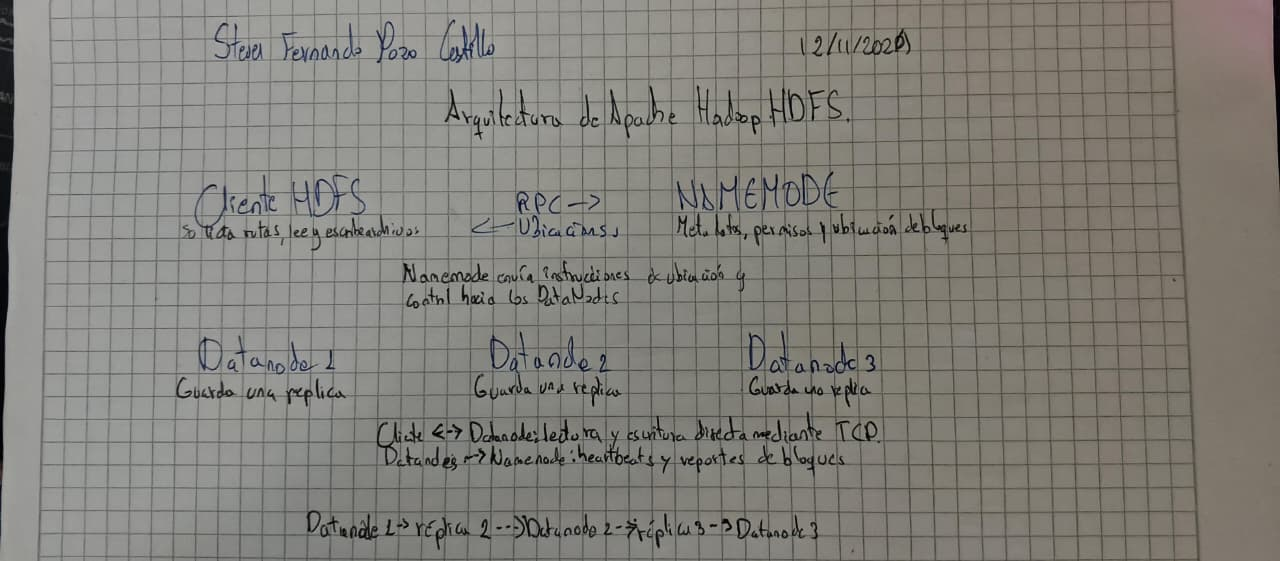
\includegraphics[width=0.98\linewidth]{../figuras/anexo_a_esquema_mano.png}
  \caption{Bosquejo inicial de la arquitectura de Apache Hadoop HDFS.}
  \label{fig:esquema-mano}
\end{figure}

\end{document}
